
%%%%%%%%%%%%%%%%%%%%%%%%%%%%%%%%%%%%%%%%%%%%%%%%%%%%%%%%
%
% Copyright (c) 2003-2010 by University of Queensland
% Earth Systems Science Computational Center (ESSCC)
% http://www.uq.edu.au/esscc
%
% Primary Business: Queensland, Australia
% Licensed under the Open Software License version 3.0
% http://www.opensource.org/licenses/osl-3.0.php
%
%%%%%%%%%%%%%%%%%%%%%%%%%%%%%%%%%%%%%%%%%%%%%%%%%%%%%%%%

\begin{figure}[t]
\centerline{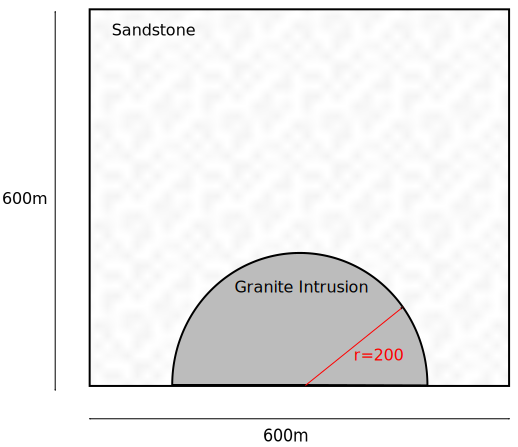
\includegraphics[width=4.in]{figures/twodheatdiff}}
\caption{Example 3: 2D model: granitic intrusion of sandstone country rock}
\label{fig:twodhdmodel}
\end{figure}

\sslist{example03a.py and cblib.py}

Building upon our success from the 1D models, it is now prudent to expand our
domain by another dimension. 
For this example we use a very simple magmatic intrusion as the basis for our
model. The simulation will be a single event where some molten granite has
formed a cylindrical dome at the base of some cold sandstone country rock.
Assuming that the cylinder is very long
we model a cross-section as shown in \reffig{fig:twodhdmodel}. We will implement
the same 
diffusion model as we have used for the granite blocks in \refSec{Sec:1DHDv00}
but will add the second spatial dimension and show how to define 
variables depending on the location of the domain. 
We use \file{onedheatdiff001b.py} as the starting point to develop this model. 

\section{Example 3: Two Dimensional Heat Diffusion for a basic Magmatic
Intrusion}
\label{Sec:2DHD}

To expand upon our 1D problem, the domain must first be expanded. In fact, we
have solved a two dimensional problem already but essentially ignored the second
dimension. In our definition phase we create a square domain in $x$ and
$y$\footnote{In \esc the notation
$x\hackscore{0}$ and $x\hackscore{1}$ is used for $x$ and $y$, respectively.}
that is $600$ meters along each side \reffig{fig:twodhdmodel}. Now we set the
number of discrete spatial cells to $150$ in both directions and the radius of
the intrusion to $200$ meters with the centre located at the $300$ meter mark
on the $x$-axis. Thus, the domain variables are;
\begin{python}
mx = 600*m #meters - model length
my = 600*m #meters - model width
ndx = 150 #mesh steps in x direction 
ndy = 150 #mesh steps in y direction
r = 200*m #meters - radius of intrusion
ic = [300*m, 0] #coordinates of the centre of intrusion (meters)
qH=0.*J/(sec*m**3) #our heat source temperature is zero
\end{python}
As before we use 
\begin{python}
model = Rectangle(l0=mx,l1=my,n0=ndx, n1=ndy)
\end{python}
to generate the domain. 

There are two fundamental changes to the PDE that we have discussed in
\refSec{Sec:1DHDv00}. Firstly,
because the material coefficients for granite and sandstone are different, we
need to deal with 
PDE coefficients which vary with their location in the domain. Secondly, we
need to deal with the second spatial dimension. We can investigate these two
modifications at the same time. 
In fact, the temperature model \refEq{eqn:hd} we utilised in
\refSec{Sec:1DHDv00} applied for the 
1D case with a constant material parameter only. For the more general case
examined in this chapter, the correct model equation is 
\begin{equation}
\rho c\hackscore p \frac{\partial T}{\partial t} -  \frac{\partial }{\partial x}
\kappa \frac{\partial T}{\partial x} -  \frac{\partial }{\partial y} \kappa
\frac{\partial T}{\partial y} = q\hackscore H 
\label{eqn:hd2}
\end{equation}
Notice that for the 1D case we have $\frac{\partial T}{\partial y}=0$ and
for the case of constant material parameters $\frac{\partial }{\partial x}
\kappa = \kappa  \frac{\partial }{\partial x}$ thus this new equation coincides
with a simplified model equation for this case. It is more convenient 
to write this equation using the $\nabla$ notation as we have already seen in
\refEq{eqn:commonform nabla};
\begin{equation}\label{eqn:Tform nabla}
\rho c\hackscore p \frac{\partial T}{\partial t} 
-\nabla \cdot \kappa \nabla T = q\hackscore H
\end{equation}
We can easily apply the backward Euler scheme as before to end up with 
\begin{equation}
\frac{\rho c\hackscore p}{h} T^{(n)} -\nabla \cdot \kappa \nabla T^{(n)}  =
q\hackscore H +  \frac{\rho c\hackscore p}{h} T^{(n-1)}
\label{eqn:hdgenf2}
\end{equation}
which is very similar to \refEq{eqn:hdgenf} used to define the temperature
update in the simple 1D case. 
The difference is in the second order derivative term
$\nabla \cdot \kappa \nabla T^{(n)}$. Under the light of the more general case
we need to revisit the \esc PDE form as shown in \ref{eqn:commonform2D}.
For the 2D case with variable PDE coefficients the form needs to be read as 
\begin{equation}\label{eqn:commonform2D 2}
-\frac{\partial }{\partial x} A\hackscore{00}\frac{\partial u}{\partial x} 
-\frac{\partial }{\partial x} A\hackscore{01}\frac{\partial u}{\partial y} 
-\frac{\partial }{\partial y} A\hackscore{10}\frac{\partial u}{\partial x} 
-\frac{\partial }{\partial x} A\hackscore{11}\frac{\partial u}{\partial y} 
+ Du = f
\end{equation}
So besides the settings $u=T^{(n)}$, $D = \frac{\rho c \hackscore{p}}{h}$ and
$f = q \hackscore{H} + \frac{\rho c\hackscore p}{h} T^{(n-1)}$ as we have used
before (see \refEq{ESCRIPT SET}) we need to set
\begin{equation}\label{eqn: kappa general}
A\hackscore{00}=A\hackscore{11}=\kappa; A\hackscore{01}=A\hackscore{10}=0
\end{equation}
The fundamental difference to the 1D case is that $A\hackscore{11}$ is not set
to zero but $\kappa$,
which brings in the second dimension. It is important to note that the
coefficients of the PDE may depend on their location in the domain which does
not influence the usage of the PDE form. This is very convenient as we can
introduce spatial dependence to the PDE coefficients without modification to
the way we call the PDE solver. 

A very convenient way to define the matrix $A$ in \refEq{eqn: kappa general}
can be carried out using the Kronecker $\delta$ symbol\footnote{see
\url{http://en.wikipedia.org/wiki/Kronecker_delta}}. The 
\esc function \verb|kronecker| returns this matrix;
\begin{equation}
\verb|kronecker(model)| = \left[ 
\begin{array}{cc}
 1 & 0 \\
 0 & 1 \\
\end{array}
\right]
\end{equation}
As the argument \verb|model| represents a two dimensional domain the matrix is
returned as a $2 \times 2$ matrix
(in the case of a three-dimensional domain a $3 \times 3$ matrix is returned).
The call 
\begin{python}
mypde.setValue(A=kappa*kronecker(model),D=rhocp/h)
\end{python}
sets the PDE coefficients according to \refEq{eqn: kappa general}.  

We need to check the boundary conditions before we turn to the question: how do
we set $\kappa$. As pointed out \refEq{NEUMAN 2} makes certain assumptions on
the boundary conditions. In our case these assumptions translate to;
\begin{equation}
-n \cdot \kappa \nabla T^{(n)} = 
-n\hackscore{0} \cdot \kappa \frac{\partial T^{(n)}}{\partial x} -
n\hackscore{1} \cdot  \kappa \frac{\partial T^{(n)}}{\partial y} = 0
\label{eq:hom flux}
\end{equation}
which sets the normal component of the heat flux $- \kappa \cdot (\frac{\partial
T^{(n)}}{\partial x}, \frac{\partial T^{(n)}}{\partial y})$ to zero. This means
that the region is insulated which is what we want. 
On the left and right face of the domain where we have
$(n\hackscore{0},n\hackscore{1} ) = (\mp 1,0)$ 
this means $\frac{\partial T^{(n)}}{\partial x}=0$ and on the top and bottom on
the domain 
where we have  $(n\hackscore{0},n\hackscore{1} ) = (\pm 1,0)$ this is
$\frac{\partial T^{(n)}}{\partial y}=0$. 

\section{Setting variable PDE Coefficients}
Now we need to look into the problem of how we define the material coefficients
$\kappa$ and $\rho c\hackscore p$ depending on their location in the domain. 
We can make use of the technique used in the granite block example in
\refSec{Sec:1DHDv00}
to set up the initial temperature. However,
the situation is more complicated here as we have to deal with a
curved interface between the two sub-domains.

Prior to setting up the PDE, the interface between the two materials must be
established. 
The distance $s\ge 0$ between two points $[x,y]$ and
$[x\hackscore{0},y\hackscore{0}]$ in Cartesian coordinates is defined as:
\begin{equation}
 (x-x\hackscore{0})^{2}+(y-y\hackscore{0})^{2} = s^{2}
\end{equation}
If we define the point $[x\hackscore{0},y\hackscore{0}]$ as $ic$ which denotes
the centre of the semi-circle of our intrusion, then for all the points $[x,y]$
in our model we can calculate a distance to $ic$. 
All the points that fall within the given radius $r$ of our intrusion will have
a corresponding 
value $s < r$ and all those belonging to the country rock will have a value $s >
r$. By subtracting $r$ from both of these conditions we find $s-r < 0$ for all
intrusion points and $s-r > 0$ for all country rock points. 
Defining these conditions within the script is quite simple and is done using
the following command:
\begin{python}
bound = length(x-ic)-r #where the boundary will be located
\end{python}
This definition of the boundary can now be used with the \verb|whereNegative|
command again to help define the material constants and temperatures in our
domain. 
If \verb|kappai| and \verb|kappac| are the 
thermal conductivities for the intrusion material granite and for the
surrounding sandstone, then we set; 
\begin{python}
x=Function(model).getX()
bound = length(x-ic)-r
kappa = kappai * whereNegative(bound) + kappac * (1-whereNegative(bound))
mypde.setValue(A=kappa*kronecker(model))
\end{python}
Notice that we are using the sample points of the \verb|Function| function space
as expected for the PDE coefficient \verb|A|\footnote{For the experienced user: use
\texttt{x=mypde.getFunctionSpace("A").getX()}.}.
The corresponding statements are used to set $\rho c\hackscore p$. 

Our PDE has now been properly established. The initial conditions for
temperature are set out in a similar manner:
\begin{python}
#defining the initial temperatures.
x=Solution(model).getX()
bound = length(x-ic)-r
T= Ti*whereNegative(bound)+Tc*(1-whereNegative(bound))
\end{python}
where \verb|Ti| and \verb|Tc| are the initial temperature in the regions of the
granite and surrounding sandstone, respectively. It is important to
notice that we reset \verb|x| and \verb|bound| to refer to the appropriate 
sample points of a PDE solution\footnote{For the experienced user: use
\texttt{x=mypde.getFunctionSpace("r").getX()}.}.

\begin{figure}[ht]
\centerline{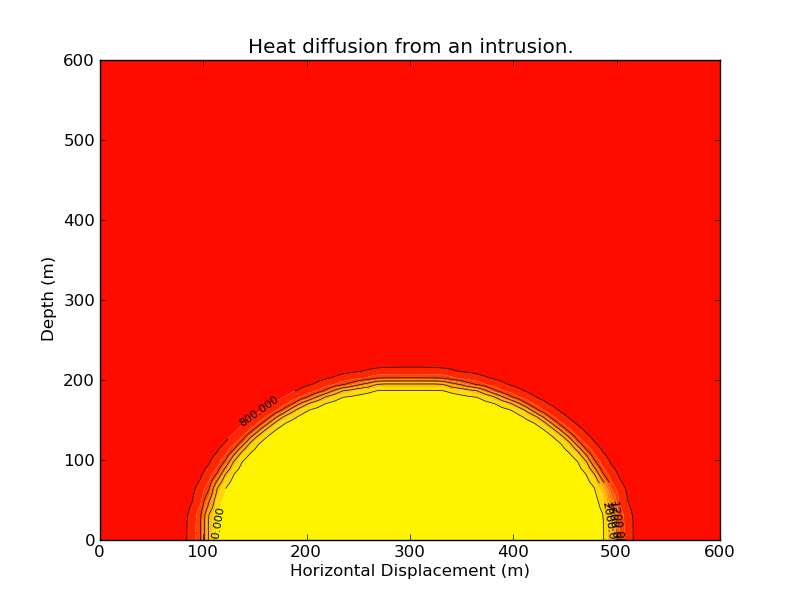
\includegraphics[width=4.in]{figures/heatrefraction001.png}}
\centerline{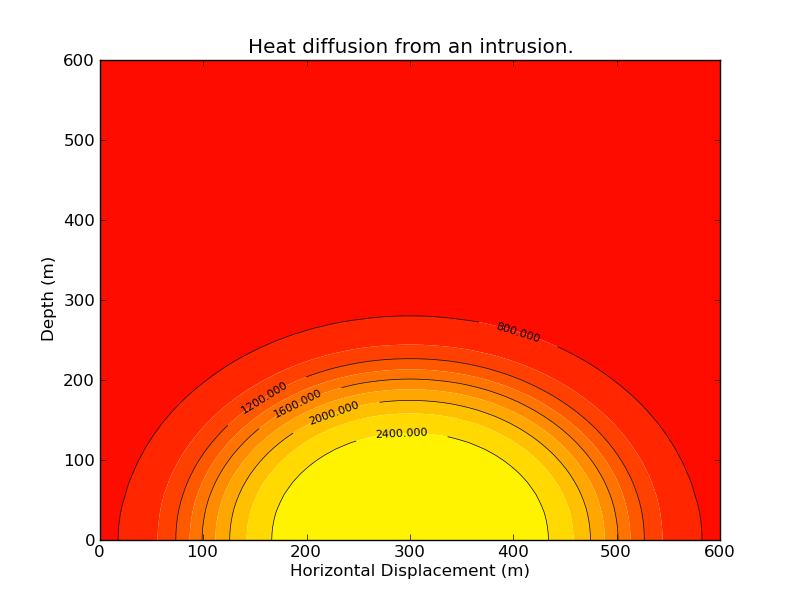
\includegraphics[width=4.in]{figures/heatrefraction030.png}}
\centerline{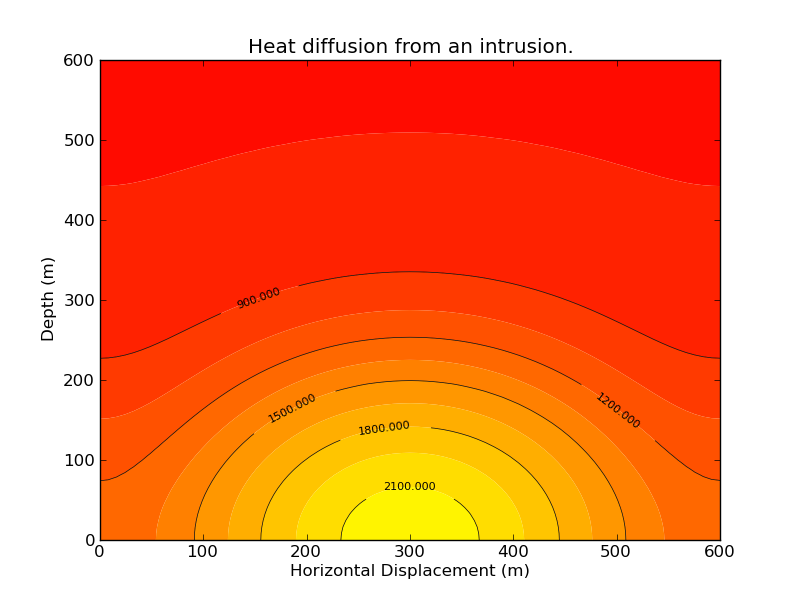
\includegraphics[width=4.in]{figures/heatrefraction200.png}}
\caption{Example 3a: 2D model: Total temperature distribution ($T$) at time step
$1$, $20$ and $200$. Contour lines show temperature.}
\label{fig:twodhdans}
\end{figure}

\section{Contouring \esc Data using \modmpl.}
\label{Sec:2DHD plot}
To complete our transition from a 1D to a 2D model we also need to modify the 
plotting procedure. As before we use \modmpl to do the plotting in this case a
contour plot. For 2D contour plots \modmpl expects that the data are regularly
gridded. We have no control over the location and ordering of the sample points
used to represent the solution. Therefore it is necessary to interpolate our
solution onto a regular grid.

In \refSec{sec: plot T} we have already learned how to extract the $x$
coordinates of sample points as 
\verb|numpy| array to hand the values to \modmpl. This can easily be extended
to extract both the $x$ and the $y$ coordinates;
\begin{python}
import numpy as np
def toXYTuple(coords):
    coords = np.array(coords.toListOfTuples()) #convert to Tuple
    coordX = coords[:,0] #X components.
    coordY = coords[:,1] #Y components.
    return coordX,coordY
\end{python}
For convenience we have put this function into \file{clib.py} so we can use
this function in other scripts more easily. 

We now generate a regular $100 \times 100$ grid over the domain ($mx$ and $my$ 
are the dimensions in the $x$ and $y$ directions) which is done using the
\modnumpy function \verb|linspace|.
\begin{python}
from clib import toXYTuple
# get sample points for temperature as  for contouring      
coordX, coordY = toXYTuple(T.getFunctionSpace().getX())
# create regular grid
xi = np.linspace(0.0,mx,75)
yi = np.linspace(0.0,my,75)
\end{python}
The values \verb|[xi[k], yi[l]]| are the grid points.

The remainder of our contouring commands resides within a \verb|while| loop so
that a new contour is generated for each time step. For each time step the
solution must be re-gridded for \modmpl using the \verb|griddata| function. This
function interprets irregularly located values \verb|tempT| at locations defined
by \verb|coordX| and \verb|coordY| as values at the new coordinates of a
rectangular grid defined by
\verb|xi| and \verb|yi|. The output is \verb|zi|. It is now possible to use the
\verb|contourf| function which generates colour filled contours. The colour
gradient of our plots is set via the command 
\verb|pl.matplotlib.pyplot.autumn()|, other colours are listed on the \modmpl web page\footnote{see
\url{http://matplotlib.sourceforge.net/api/}}. Our results are then contoured,
visually adjusted using the \modmpl functions and then saved to a file.
\verb|pl.clf()| clears the figure in readiness for the next time iteration.
\begin{python}
#grid the data.
zi = pl.matplotlib.mlab.griddata(coordX,coordY,tempT,xi,yi)
# contour the gridded data, plotting dots at the randomly spaced data points.
pl.matplotlib.pyplot.autumn()
pl.contourf(xi,yi,zi,10)
CS = pl.contour(xi,yi,zi,5,linewidths=0.5,colors='k')
pl.clabel(CS, inline=1, fontsize=8)
pl.axis([0,600,0,600])
pl.title("Heat diffusion from an intrusion.")
pl.xlabel("Horizontal Displacement (m)")
pl.ylabel("Depth (m)")
pl.savefig(os.path.join(save_path,"Tcontour%03d.png") %i)
pl.clf()        
\end{python}
The function \verb|pl.contour| is used to add labelled contour lines to the
plot. 
The results for selected time steps are shown in \reffig{fig:twodhdans}.


\section{Advanced Visualisation using VTK}

\sslist{example03b.py}
An alternative approach to \modmpl for visualisation is the usage of a package
which is based on the Visualization Toolkit (VTK) library\footnote{see \url{http://www.vtk.org/}}.
There is a variety of packages available. Here we use the package \mayavi\footnote{see
\url{http://code.enthought.com/projects/mayavi/}} as an example. 

\mayavi is an interactive, GUI driven tool which is 
really designed to visualise large three dimensional data sets where \modmpl 
is not suitable. But it is also very useful when it comes to two dimensional
problems. 
The decision of which tool is the best can be subjective and users should
determine which package they require and are most comfortable with. The main
difference between using \mayavi (or other VTK based tools) and \modmpl is that
the actual visualisation is detached from the calculation by writing the
results to external files and importing them into \mayavi. In 3D the best
camera position for rendering a scene is not obvious before the results are
available. Therefore the user may need to try different settings before the
best is found. Moreover, in many cases a 3D interactive visualisation is the
only way to really understand the results (e.g. using stereographic projection).

To write the temperatures at each time step to data files in the VTK file format
one needs to insert a \verb|saveVTK| call into the code;
\begin{python}
while t<=tend:
      i+=1 #counter
      t+=h #current time
      mypde.setValue(Y=qH+T*rhocp/h)
      T=mypde.getSolution()
      saveVTK(os.path.join(save_path,"data.%03d.vtu"%i, T=T)
\end{python}
The data files, e.g. \file{data.001.vtu}, contain all necessary information to 
visualise the temperature and can be directly processed by \mayavi. Note that
there is no re-gridding required. It is recommended to use the file extension
\file{.vtu} for files created by \verb|saveVTK|. 

\begin{figure}[ht]
\centerline{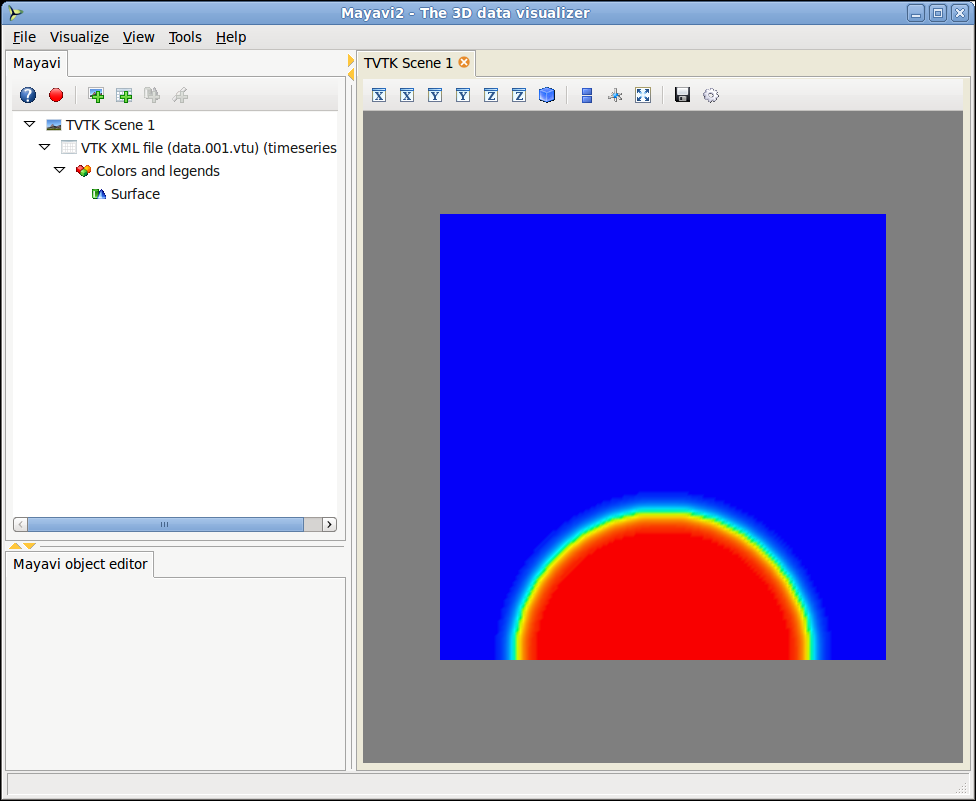
\includegraphics[width=4.in]{figures/ScreeshotMayavi2n1}}
\caption{Example 3b: \mayavi start up window}
\label{fig:mayavi window}
\end{figure}

\begin{figure}[ht]
\centerline{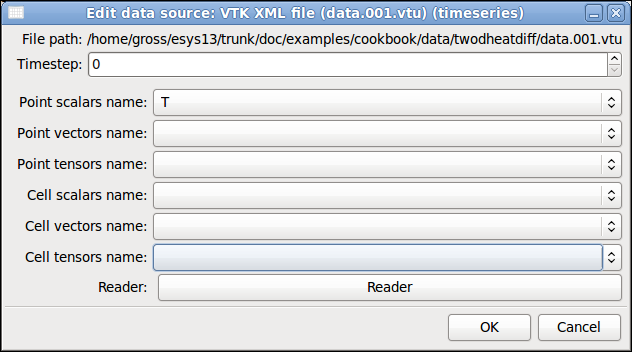
\includegraphics[width=4.in]{figures/ScreeshotMayavi2n2}}
\caption{Example 3b: \mayavi data control window}
\label{fig:mayavi window2}
\end{figure}
After you run the script you will find the 
result files \file{data.*.vtu} in the result directory \file{data/example03}.
Run the command
\begin{python}
>> mayavi2 -d data.001.vtu -m Surface &
\end{python}
from the result directory. \mayavi will start up a window similar to
\reffig{fig:mayavi window}.
The right hand side shows the temperature at the first time step. To show
the results at other time steps you can click at the item \texttt{VTK XML file
(data.001.vtu) (timeseries)}
at the top left hand side. This will bring up a new window similar to the window
shown in \reffig{fig:mayavi window2}. By clicking at the arrows in the top
right corner you can move forwards and backwards in time. 
You will also notice the text \textbf{T} next to the item \texttt{Point scalars
name}. The
name \textbf{T} corresponds to the keyword argument name \texttt{T} we have
used in the \verb|saveVTK| call. In this menu item you can select other results
you may have written to the output file for visualisation.

\textbf{For the advanced user}: Using the \modmpl to visualise spatially
distributed data is not MPI compatible. However, the \verb|saveVTK| function
can be used with MPI. In fact, the function collects the values of the sample
points spread across processor ranks into a single file.
For more details on writing scripts for parallel computing please consult the
\emph{user's guide}.

